\documentclass[a4paper]{article}
\usepackage[T1]{fontenc}
\usepackage[utf8x]{inputenc}
\usepackage[english,russian]{babel}
\usepackage{multicol}
\usepackage{fancyhdr}
\usepackage[warn]{mathtext}
\usepackage{graphicx}
\usepackage{microtype}
\usepackage{wrapfig}
\usepackage{amsmath}
\usepackage{floatflt}
\usepackage{geometry} \geometry{verbose,a4paper,tmargin=2cm,bmargin=2cm,lmargin=1.5cm,rmargin=1.5cm}
\usepackage{float}
\usepackage{amssymb}
\usepackage{caption}
\usepackage{epsfig}
\usepackage{newunicodechar}
\usepackage{manfnt}
\usepackage{wasysym}

\begin{document}
\newcommand{\apple}{\char"F8FF}

\begin{titlepage}
	\centering
	\vspace{5cm}
    {\scshape\LARGE Московский физико-технический институт\par}
    

	\vspace{8cm}
	{\scshape\Large Лабораторная работа по общей физике \par}
	\vspace{2cm}
    {\huge\bfseries  2.1 Опыт Франка-Герца  \par}
	\vspace{4cm}
	\vfill
\begin{flushright}
	{\large выполнил студент Б04-852 группы ФЭФМ}\par
	\vspace{0.3cm}
	{\LARGE Яромир Водзяновский}
\end{flushright}
	
	\vfill
Долгопрудный, 2020
% Bottom of the page
\end{titlepage}

\pagestyle{fancy} 
\fancyhead{}
\fancyhead[R]{Опыт Франка-Герца}
\fancyhead[L]{Квантовая физика $\sim  \hat(\, ^{\circ} \omega  ^{\circ} \, \hat) \sim$}
% \fancyhead[LE,RO]{Квантовая физика   $ (^{/} \hat\; \omega  \hat\;) ^{/}$}
\fancyhead[C]{}
\fancyfoot[C]{ \noindent\rule{\textwidth}{0.4pt} \thepage }
% $\sim(\; ^{\circ }\omega   \; ) \sim$

\newpage


\section{Цель работы}

Методом электроннорго возбуждения измерить энергию первого уровня атома гелия в динамическом 
и статическом режимах.

\section{Оборудование}
\begin{enumerate}
    \item Трехэлектродная лампа ЛМ-2
    \item Батарея 4.5 В
    \item Микроамперметр
    \item Понижаюзщий трансформатор
    \item Осциллограф
    \item Блок источников питания
    \item Вольтметр В7-22А
\end{enumerate}


\section{Теория}

Опыт Франка-Герца подтверждает существование дискретных уровней энергий атомов.

Разреженный одноатомный газ заполняет трехэлектродную лампу рис.\ref{p1}. Передвигаясь от катода к аноду 
электроны сталкиваются с атомами гелия и могут ионизировать или возбудить атом или упруго соудариться.

Энергия электрона увеличивается с ростом разности потенциалов между катодом и анодом и достигает 
величины для возбуждения атома. При таком неупругом соударении энергия электрона передается атому 
и электрон переходит на более высокий уровень или совсем отрывается (ионизация).

Потенциал коллектора немного меньше чем у анода, значит есть сдерживающее поле. Ток коллектора $\sim$ 
количеству падающих на него электронов.

\begin{figure}[h]
	\begin{center}
	\begin{minipage}[h]{0.45\linewidth}
	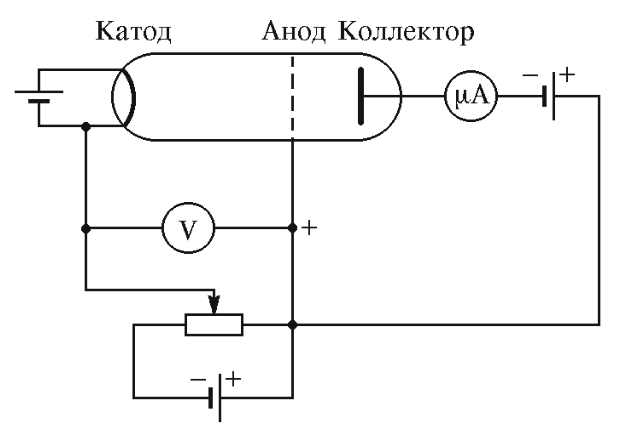
\includegraphics[width=1\linewidth]{p1.png}
	\caption{Принципиальная схема опыта Франка-Герца} 
	\label{p1}
	\end{minipage}
	\hfill 
	\begin{minipage}[h]{0.45\linewidth}
	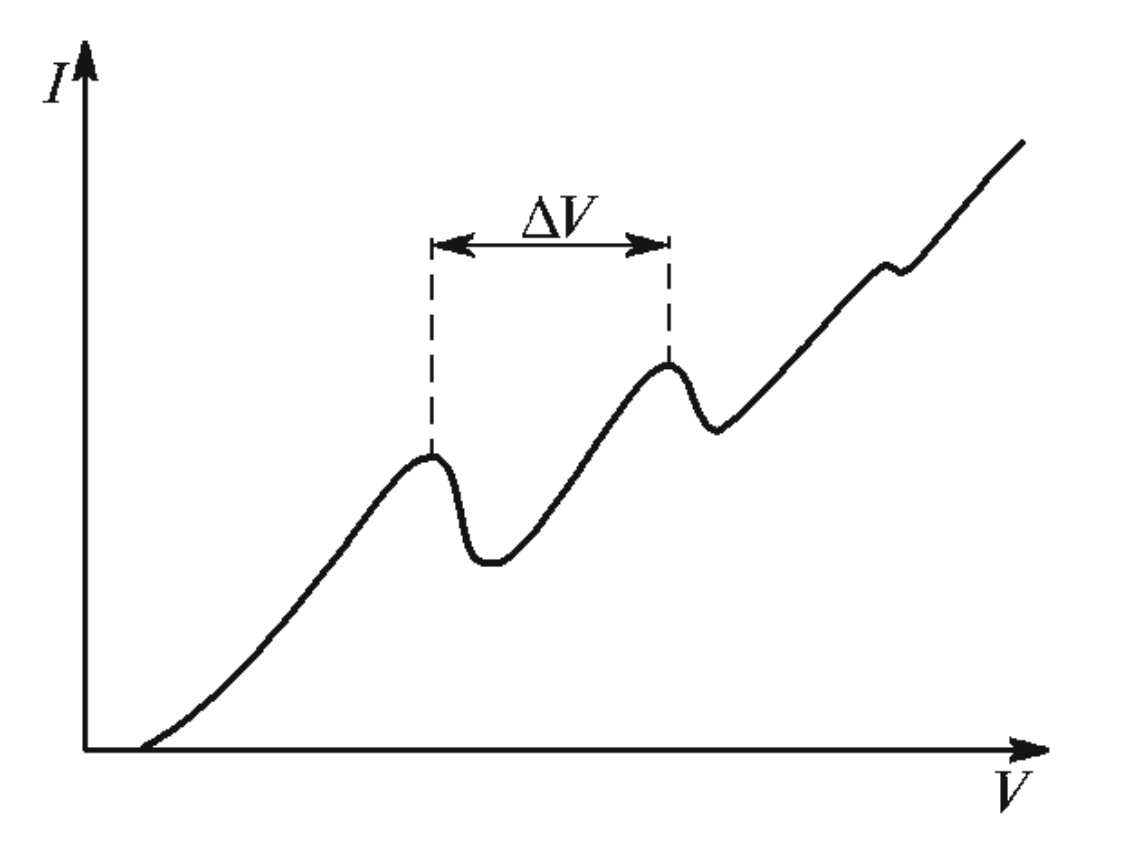
\includegraphics[width=1\linewidth]{p2.png}
	\caption{Зависимость тока коллектора от напряжения на аноде}
	\label{p2}
	\end{minipage}
	\end{center}
\end{figure}

При увеличении потенциала анода ток в лампе вначале растет как в вакуумном диоде. Когда энергия электронов
достаточна для вощбуждения, то ток коллектора резко падает, тк электроны теряют почти всю энергию и 
не могу преодолеть задерживающий потенциал $\sim 1$В. При дальнейшем росте потенциала анода ток коллектора 
вновь растет.

Следующее замедление просиходит, когда электроны дважды сталкиваются с атомами, по середине и у анода.
Ряд максимумов и минимумов на расстояниях $\Delta V \sim $ энергии первого возбужденного состояния.

При более точной установке можно было бы увидеть и тонкую структуру кривой распада тока, содержащую 
ряд минимумов, соответствующих возбуждению других уровней, но это уже совсем другая история :)

\section{Экспериментальная установка}

Схема Экспериментальной установки изображена на рис.\ref{setup}. Используется серийная лампа ионизационного
манометра ЛМ-2, заполненная гелием $\sim 1$ Торр. 

\begin{figure}[H]
	\begin{center}
	\begin{minipage}[h]{0.4\linewidth}
	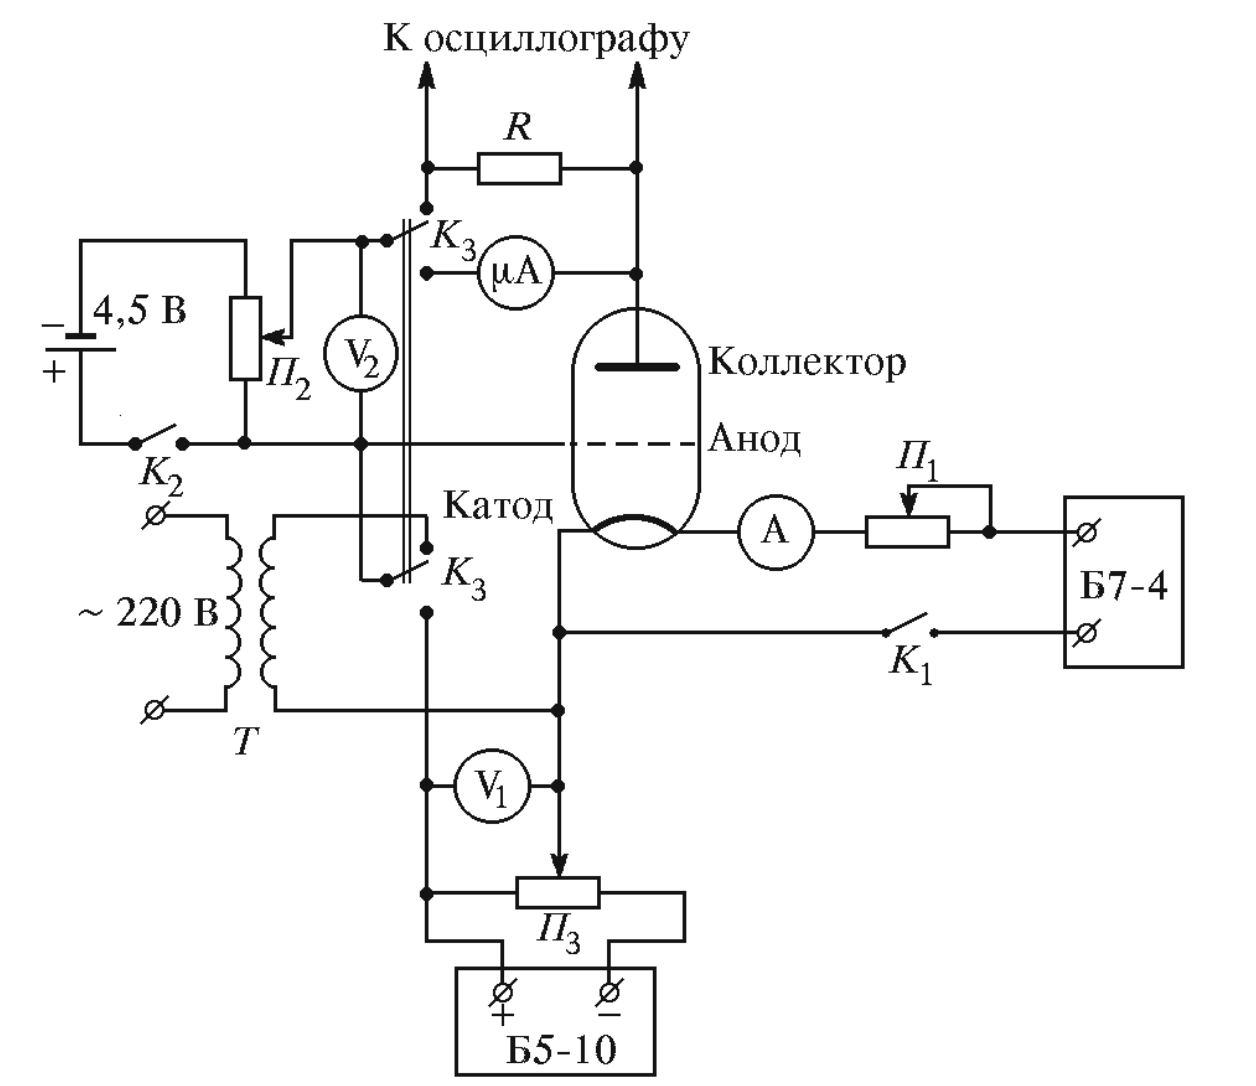
\includegraphics[width=1\linewidth]{setup.png}
	\caption{Схема экспериментальной установки} 
	\label{setup}
	\end{minipage}
	\hfill 
	\begin{minipage}[h]{0.59\linewidth}
	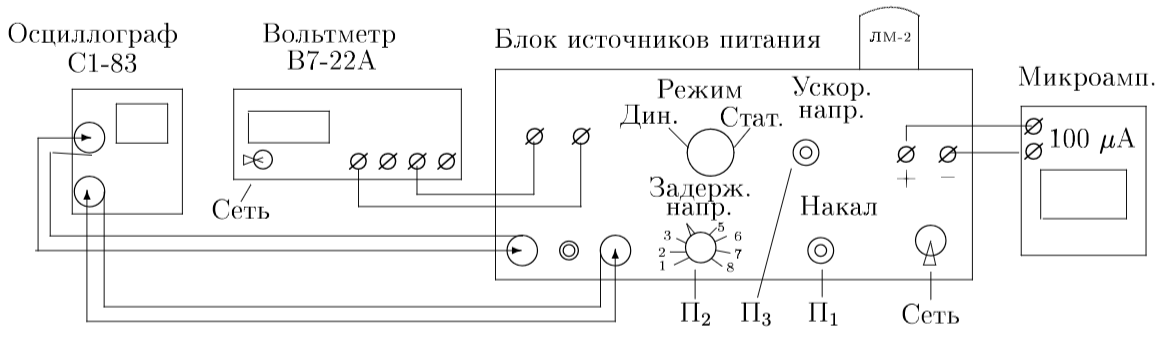
\includegraphics[width=1\linewidth]{block.png}
	\caption{Блок-схема}
	\label{block}
    \end{minipage}
	\end{center}
\end{figure}

На рис.3 обозначены:
\begin{itemize}
    \item А - амперметр
    \item Б7-4 - стабилизированный источник питания (подаёт напряжение накала)
    \item $K_1$ - тумблер для включения в цепь источника Б7-4
    \item Б5-10 - выпрямитель (подаёт на анод ускоряющее напряжение)
    \item $\Pi_3$ - потенциометр, регулирующий величину ускоряющего напряжения
    \item $V_1$ - вольтметр, измеряющий величину ускоряющего напряжения
    \item 4,5 В - источник задерживающего потенциала
    \item $\Pi_2$ - потенциометр, регулирующий величину задерживающего потенциала
    \item $V_2$ - вольтметр, измеряющий величину задерживающего потенциала
    \item $\mu A$ - микроамперметр - регистрирует ток в цепи коллектора
    \item $K_3$ - ключ, переключающий схему из статического режима в динамический
    \item Т - понижающий трансформатор - подаёт ускоряющий потенциал при динамическом режиме
    \item R - нагрузочный резистор
\end{itemize}

Есть 2 режима измерений: \par
	\textbf{-} При динамическом режиме ускоряющий потенциал подается с понижающего трансформатора
	а ток коллектора регистрируется осциллографом, подключенным к нагрузочному резистору $R$. \par
	\textbf{-} При статическом режиме напряжение $V_a$ между анодом и катодом измеряется вольтметром
	И7-22А, подключенным к клеммам "Вольтметр". Ток коллектора измеряется микроамперметром. 

Заметим, что при определении энергии электронов по разности потенциалов между анодом и катодом стоит учесть 
контактную разность потенциалов и первый максимум не соответсвует потенциалу первого возбужденного уровня. 
однако контактная разность потенциалов сдвигает все максимумы одинаково. 


\section{Ход работы}

\subsection{Получение ВАХ $I_k = f(V_a)$ на экране осциллографа С1-83}

\begin{enumerate}
	\item Поставим ручку "Режим" в положение "Динамич".
	\item Установим ручку "Накал" на максимум.
	\item При максимальном ускоряющем напряжении измерим на экране расстояние между максимумами
	и между минимумами осциллограммы. Повторим это для 3-х задерживающих напряжений: 4, 6 и 8 В.
	\item Сфотографируем осциллограммы для 3-х значений задерживающего напряжения.
	
	\begin{figure}[H]
		\begin{center}
		\begin{minipage}[h]{0.3\linewidth}
		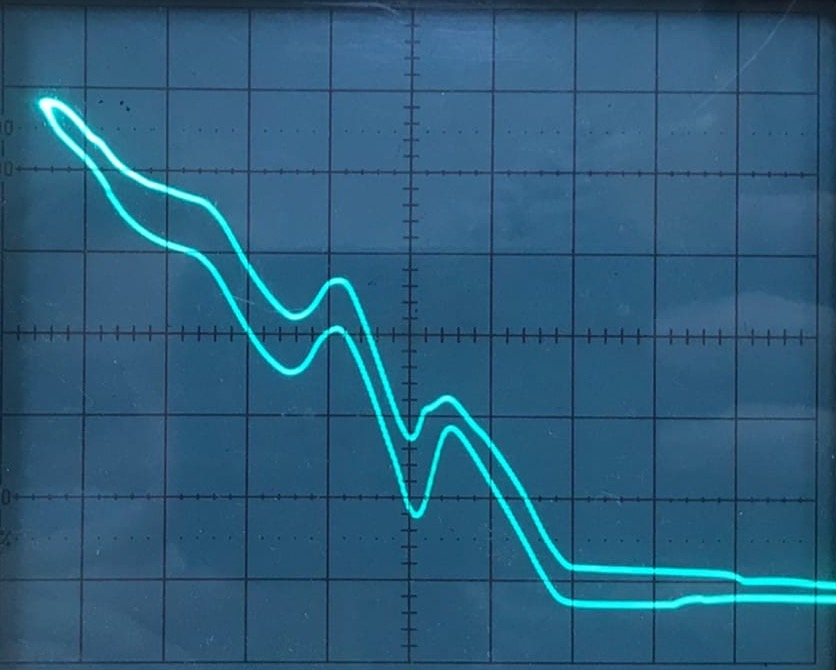
\includegraphics[width=1\linewidth]{4.jpg}
		\caption{Задерживающее напряжение 4 В} 
		\label{4v}
		\end{minipage}
		\hfill 
		\begin{minipage}[h]{0.3\linewidth}
		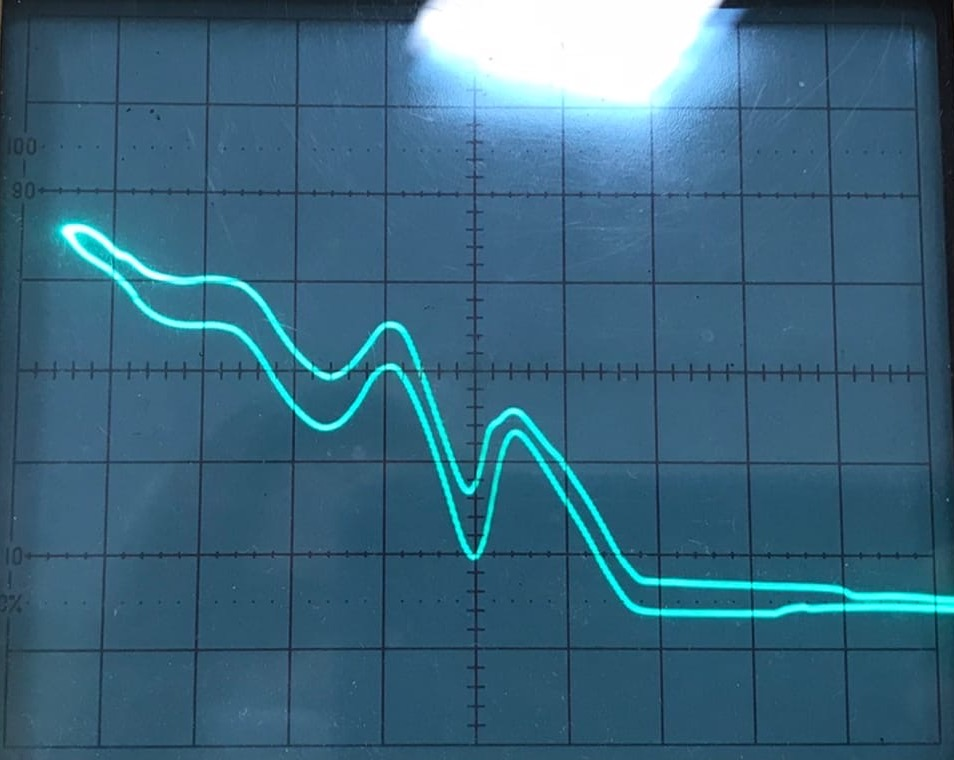
\includegraphics[width=1\linewidth]{6.jpg}
		\caption{Задерживающее напряжение 6 В}
		\label{6v}
		\end{minipage}
		\hfill 
		\begin{minipage}[h]{0.3\linewidth}
		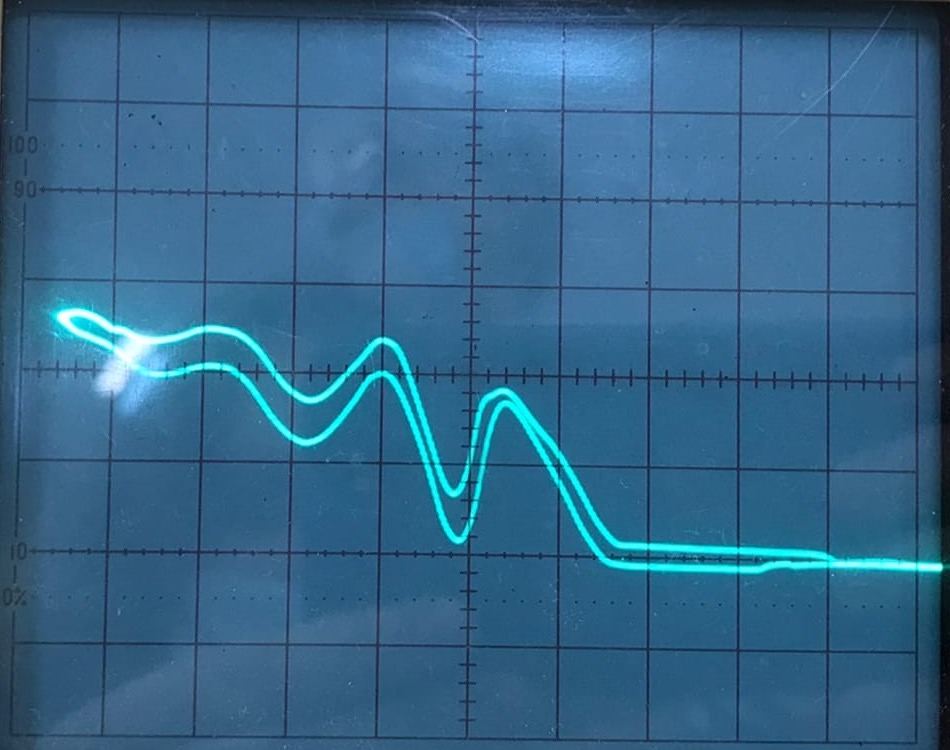
\includegraphics[width=1\linewidth]{8.jpg}
		\caption{Задерживающее напряжение 8 В}
		\label{8v}
		\end{minipage}
		\end{center}
	\end{figure}

	\item По фотографиям опредлим максимумы и минумумы напряжения, знасем в таблицу ниже
	
	\begin{table}[H]
		\centering
		\begin{center}
		\end{center}
		\vspace{0.1cm}
		\begin{tabular}{ |p{3.5cm}||p{1cm}|p{1cm}|p{1cm}|p{1cm}|p{2.5cm}|p{1cm}|p{1cm}|}
	 \hline
	Задерж. напряжение, В & $V_{min_1}$, дел & $V_{min_2}$, дел & $V_{max_1}$, дел & $V_{max_2}$, дел & Погрешность, дел & $\triangle V_{min}$, дел & $\triangle V_{max}$, дел\\
	 \hline
	 4  & -7 & 0 & -4.5 & 2.5 & 1  & 7 & 7\\
	\hline
	 6  & -8 & 0 & -4.5 & 2 & 1  & 8 & 6.5\\
	\hline
	 8  & -9 & -1.5 & -5 & 2 & 1  & 7.5 & 7\\
	\hline
	\end{tabular}
	\end{table}


	Определим средние значения:

	$$\Delta V_{max} = 6.83 \pm 1.04 (\text{дел}) \pm 15.2\% \;\;\;\;\;\;\; \Delta V_{min} = 7.5 \pm 1.12 (\text{дел}) \pm 14.9\%$$

	Усредним эти значения:
	$$V = 7.17 \pm 1.52 (\text{дел}) \pm 21.3\%$$


\end{enumerate}

\subsection{Получение ВАХ $I_k = f(V_a)$ в статическом режиме}

\begin{enumerate}
	\item Переведем переключатель "Режим" в положение "Статич"
	\item Установим максимальный накал 
	\item Установим задерживающее напряжение на 4В
	\item Включим в сеть подсветку микроамперметра и вольтметр. 
	\item Плавно увлеичивая ускоряющее напряжение $V_a$ снимем ВАХ зависимость коллекторного тока от 
	анодного напряжения. Результаты занесем в таблицы на рисунках \ref{t1}, \ref{t2}, \ref{t3}.


\newpage

\begin{figure}[H]
	\begin{center}
	\begin{minipage}[h]{0.3\linewidth}
	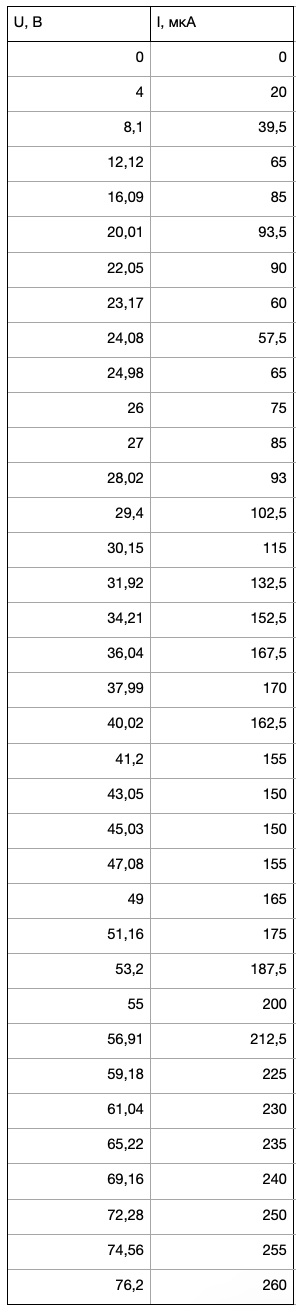
\includegraphics[width=1\linewidth]{t1.png}
	\caption{Задерживающее напряжение 4 В} 
	\label{t1}
	\end{minipage}
	\hfill 
	\begin{minipage}[h]{0.3\linewidth}
	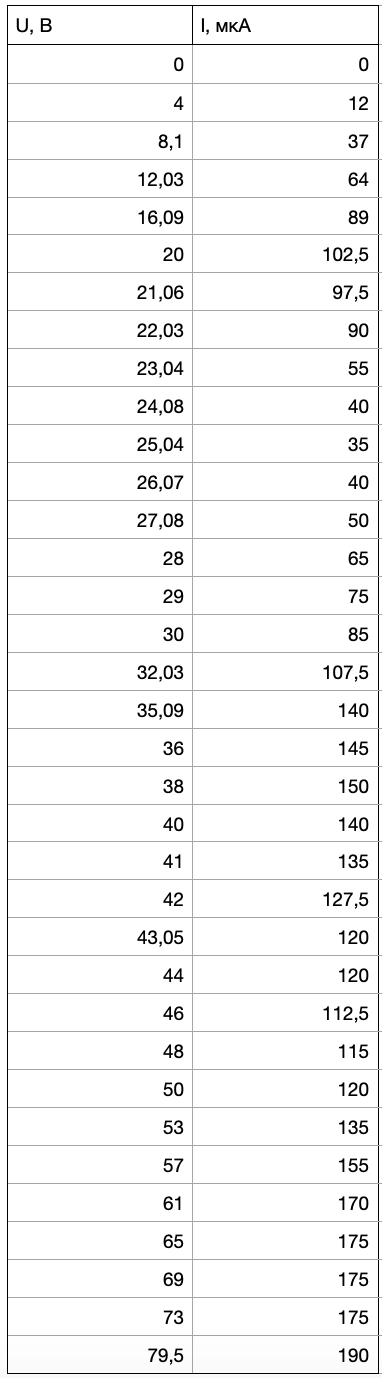
\includegraphics[width=1\linewidth]{t2.png}
	\caption{Задерживающее напряжение 6 В}
	\label{t2}
    \end{minipage}
    \hfill 
	\begin{minipage}[h]{0.3\linewidth}
	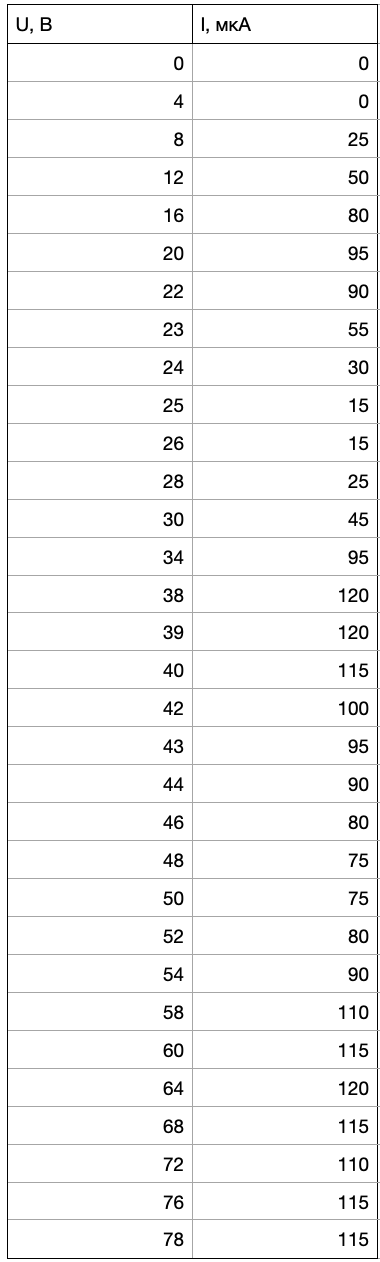
\includegraphics[width=1\linewidth]{t3.png}
	\caption{Задерживающее напряжение 8 В}
	\label{t3}
	\end{minipage}
	\end{center}
\end{figure}

\item Построим графики $I_k = f(V_a)$ при разных задерживающих напряжениях.

\begin{figure}[H]
	\begin{center}
	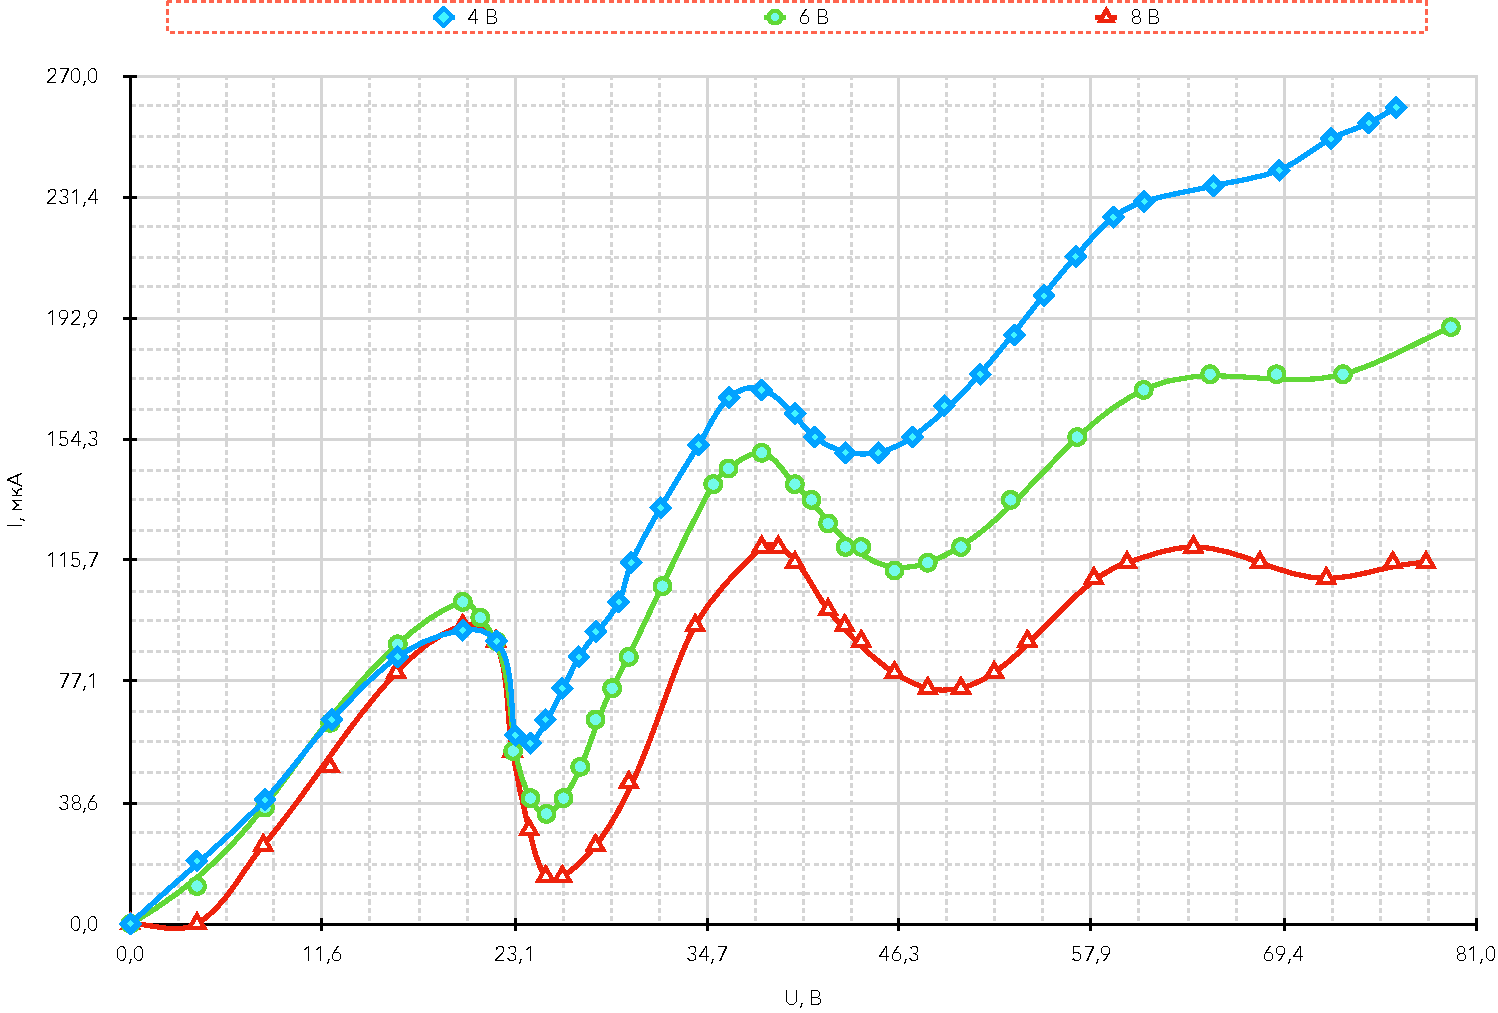
\includegraphics[scale = 0.6]{graph.pdf}
	\caption{ВАХ трехэлектронной вакуумной лампы при разных запирающих напряжениях.}
	\label{graph}
	\end{center}
\end{figure}

\item 
По графикам определим энергию возбуждения первого уровня атома гелия и занесем в таблицу ниже

\begin{table}[H]
    \centering
    \begin{center}
    \end{center}
    \vspace{0.1cm}
    \begin{tabular}{ |p{3.5cm}||p{1.5cm}|p{1.5cm}|p{1.5cm}|p{1.5cm}|p{2.5cm}|p{1.5cm}|p{1.5cm}|}
 \hline
Задерж. напряжение, В & $V_{max_1}$, В & $V_{max_2}$,В & $V_{min_1}$,В & $V_{min_2}$,В & Погрешность, В & $\triangle V_{max}$, В & $\triangle V_{min}$, В\\
 \hline
 4  & 20.5  & 37.6  & 23.83  & 49.2  & 1  & 17.1  & 25.37 \\
\hline
 6  & 20.3  & 37.86 & 24.55  & 46.3  & 1  & 17.56  & 21.75 \\
\hline
 8  & 21.01  & 37.33 & 25.73  & 44.85  & 1  & 16.32  & 19.12 \\
\hline

\end{tabular}
\end{table}

Определим средние значения:

$$\Delta V_{max} = 22.08 \pm 3.14 (B) \pm 14.2\% \;\;\;\;\;\;\; \Delta V_{min} = 16.99 \pm 0.63 (B) \pm 3.7\%$$

Усредним эти значения:
$$V = 19.53 \pm 2.87 (B) \pm 14.67\%$$

\end{enumerate}

\section{Вывод}

В ход еработы был воспроизведен опыт Франка-Герца, подтверждающий наличие дискретных уровней 
возбуждения атомов. ВАХ трехэлектронной лампы была измерена двумя способами - динамическим и 
статическим. По этим ВАХ были жкспериментально определены потенциалы возбуждения атомов гелия.

\end{document}